\documentclass{article}
\usepackage[utf8]{inputenc}

\usepackage{indentfirst}


\usepackage{amsmath}
%\usepackage[sfdefault]{roboto}
\usepackage[T1]{fontenc}
\usepackage[utf8]{inputenc}

% estabelece margens do papel
\usepackage[lmargin=3cm, tmargin=3cm,r margin=2cm, bmargin=2cm]{geometry}

% Imagens
\usepackage{wrapfig}

% adicionar suporte ao idioma pt-br
\usepackage[brazil]{babel}

% Utilização de imagens
\usepackage{graphicx} 
\usepackage{wrapfig}

% Possibilita o uso do H no posicionamento de figuras
\usepackage{float} 

% das referências
\usepackage[round]{natbib}
\bibliographystyle{dinat}
\usepackage{url}

% permite criação região de comentário
\usepackage{comment}


\begin{document}


\setcounter{page}{1}
\pagenumbering{arabic}
\newpage

\begin{center}
    {\huge  Análise da interação Hospedeiro-parasitóide}
    
    \medskip
    
    {\large Daniel Ambrosim Falqueto e Darlan Augusto Farias Araújo}
    
    \medskip
    
    FGV - Fundação Getúlio Vargas, setembro de 2022
\end{center}

\section{Resumo}

O modelo matemático hospedeiro-parasitóide é um modelo que foi desenvolvido com o objetivo de entender as interações de uma ou mais espécies de hospedeiros para um respectivo parasita que em sua maioria são Insetos. O objetivo de modelar tais interações se deve ao fato de que o controle biológico de pragas, que em sua maioria são insetos, é muito necessário já que se não houver o controle desse tipo de praga, um enorme prejuízo pode ser causado, sejam eles para própria natureza ou para o ser humano. A modelagem dessa interação permite a tomada de uma contramedida, em sua maioria um controle biológico clássico, onde o dano que esses seres causam é controlado com a adição de um inimigo natural desse parasita, que reduziria a população desse mesmo ser. Esse método é um dos mais eficientes já que não é um meio de redução químico ou não natural.

\section{Por que combinar modelagem ecológica com controle da população de pragas?}

Geralmente, os padrões de ciclos, picos ou crashes ecológicos das tendências populacionais estão fortemente associados a doenças endógenas e/
ou forças exógenas. Por isso a relção ou correlação dessas forças com a abundância populacional tem sido muito estudadas nas últimas dácadas. Além disso, o bioma terrestre passou por intensas e rápidas mudanças, principalmente desde o século passado por causa da ação humana, provavelmente resultando em novos padrões ecológicos como resultado da pressão exercida por essas mudanças nos organismos.

A expressão “mundo em mudança” está presente ou implícita em muitos jornais, revistas, jornais, ou mesmo títulos de reuniões científicas. Particularmente, na entomologia há uma crescente preocupação com o mundo em mudança associado à surtos de pragas, ruídos ambientais, invasões biológicas e o estabelecimento de espécies exóticas em novas áreas. Essa preocupação decorre da saúde humana e animal, o papel dos insetos na agricultura, juntamente com os integrantes essenciais da biodiversidade. Os efeitos das mudanças no mundo são refletidas nas dinâmicas populacionais e investigar transformações rápidas não é um trabalho trivial pelo menos para entende-los em sua totalidade.

Um modelo matemático é essencialmente uma caricatura de um sistema e pode funcionar como um importante protótipo a ser investigado, principalmente por causa de sua estrutura simples. O primeiro passo para modelar os sistemas é entender parcialmente modelos complexos, porque uma característica importante dos modelos é sua flexibilidade. Vamos tentar mostrar quais são os principais pontos listados atualmente pelos ecologistas e entomologistas, que podem impedir a compreensão do comportamento da população de insetos e, consequentemente, a implementação do Manejo Integrado de Pragas (MIP).

\section{Suprimento de comida e insetos}

Um dos maiores impecílios da humanidade em relação a produção de alimentos, tarefa que por si só é desafiadora, são as pragas. Durante vários anos a humanidade encontrou modos para lidar com essa categoria de criatura, apesar de que a maioria dos métodos resultava não só no extermínio desses seres, mas também em uma transformação drásticamente nociva no ambiente, fauna, flora e por consequência no próprio ser humano. Exemplos dessas soluções são os agrotóxicos, que apesar de fazer seu trabalho de exestermínio com sucesso, acabam por gerar um dano residual no ambiente em que são aplicados, afentando a vegetação, animais, rios, lagos e etc. Causando um ano na própria natureza que pode ser incalculável.

O deselvolvimento humano e a oferta alimentar são conceitos que devem estar de mãos dadas, porém não é isso que anda acontecendo recentemente no mundo, criando uma dependência no aumento de recursos alimentares, que por sua vez resulta em uma necessidade na redução criada pelas pragas. Além da necessidade no aumento dos niveis atuais em relação a produção de alimentos, causado pela crescente desnutrição humana no mundo inteiro.

O avanço tecnológico tem sido de grande contribuição para o aumento da eficiência da agricultura, principalmente quando se trata de alimentos trangênicos, ao usar da ciência para alterar o DNA das plantas, melhorando sua variabilidade genética, resultando em maior resistência a doenças e maior tempo de vida. Porém, mesmo isso não é necessário para controlar a enorme demanda da humanidade por alimentos, algo que gerará prejuízos futuramente. Esses fatos são colocados a mesa sem contar o prejuízo causado por pragas, o que geraria um futuro realmente péssimo na perspectiva humana.


\section{Pesticidas e MIP}

Um dos desafios desse século é tentar controlar o avanço de insetos e pragas. Uma das tentativas é o uso de pesticidas que, quando utilizados em excesso, contaminam alimentos, o meio ambiente e acabam eliminando também outros insetos que são inimigos naturais das pragas e não prejudicam a produção dos alimentos. Porém utilizar um inimigo natural especializado tem a desvantagem fundamental de que dificilmente pode erradicar a praga alvo, a menos que a primeira seja altamente vulnerável a um efeito específico. 

Por isso novas técnicas tem sido desenvolvidas, como variedades resistentes, rotação de culturas e lavouras, fertilização, saneamento, culturas com armadilhas, poda, etc. Além disso aumento e soltagem de predadores naturais, parasitóides e/ou patógenos também começaram a ser utilizados. Em particular, técnicas genéticas, como liberação de insetos estéreis e organismos modificados estão em intenso desenvolvimento para aplicação imediata. Embora a importância do novo cenário seja reconhecida a falta de dados para o modelo dificulta a modelagem precisa da utilização dos pesticidas modernos e os métodos de controle acima mencionados sobre pragas de insetos, bem como na saúde humana e no ambiente. 

Para compensar parcialmente os efeitos negativos pré-mencionados do uso de um inimigo natural especializado, uma abordagem promissora é implementar um conjunto multi-inimigo em vez de um único agente de biocontrole. A previsão é encorajadora para o uso do paradigma de assemblage multi-inimigo no manejo de pragas. No entanto, o
questão prática central, que permanece obscura, é sobre a alteração do tamanho da população do alvo
pragas após o biocontrole, ou seja, se o uso de vários agentes reduzirá bastante o impacto negativo
da praga no meio ambiente. De fato, os estudos teóricos existentes sobre as coinfecções estão principalmente focados em
a evolução da virulência, prevalência da doença ou a derivação do número básico de reprodução

\section{Aquecimento global e Insetos}
Devido ao crescente aumento do aquecimento global associado aos gases do efeito estufa, tanto fauna quanto flora se vem em constante mudança devido ao fenômeno, influenciando a demografia, geração e interação com plantas das ditas pragas, afetando então diretamente as dinâmicas hospedeiro-parasitóide, de produção de alimentos e de proliferação de doenças. Os anos se passam e os danos causadas pelas pragas aumenta, em conjunto o aquecimento global causa enormes perdas florestais, que não só podem ser concequências do fenômeno, mas também ter influência humana, isso tudo resulta no aumento da geração das pragas.
Um exemplo é o mosquito Aedes aegypti, onde foi analisado por Kearney (2009), que em diferentes regiões termicas da Australia o inseto se reproduz de maneira mais intensa. Isso pode significar que doenças transmitidas por insetos podem começar a surgir em novas áreas em decorrência das mudanças de temperatura. Isso fica mais evidente ao aumento de casos de doenças importadas como a própria dengue.


\section{Cenários, Teoria Ecológica e MIP}

A complexidade da natureza é um cenário atraente para a aplicação de raciocínios complexos e ferramentas analíticas sofisticadas. O desafio que surge é como conectar a ciência teórica com os experimentos para medir e melhorar a produção sem causar danos a natureza. A mudança ao longo do tempo das populações de insetos pode exibir padrões ecológicos que podem descrever tendências importantes que pode indicar suscetibilidade a falhas ou surtos. 
Outra questão importante é entender como e quando vai ocorrer uma explosão de insetos, algo que infelizmente é difícil de se prever. Programas de manejo populacional de pragas e insetos vêm sendo implementados há décadas na tentativa de controlar pragas. No entanto, na prática, raramente os programas incorporam todos os componentes que são necessários para avaliar periodicamente o estado das pragas. O manejo de espécies de pragas também implica a análise de padrões ecológicos investigando a frequência de distribuição de insetos para avaliar o padrão de dispersão espacial e desenvolver planos de decisão. Os planos para amostragem de populações de insetos levam em consideração pelo menos três componentes: densidade populacional das pragas, limiar econômico e a previsão dos fenômenos.

\section{Artigos com modelagem relacionada}

O artigo "Ecological Modeling and Pest Population Management" (1), explica como Tang & Cheke (2008) estenderam o clássico modelo hospedeiro-parasitóide, incluindo o programa de controle de Manejo Integrado de Pragas (MIP) para considerar o limiar econômico como um componente da formulação. Os resultados encontrados neste estudo sugerem que é possível manter o nível de host abaixo do limiar econômico (LE), evitando o nível de prejuízo econômico (NPE). Além disso, eles mostraram que uma alta densidade inicial de parasitóides, bem como alta sobrevivência intergeracional parasitóide pode influenciar o padrão ecológico da série temporal. Nos programas de MIP, geralmente tanto a pulverização de pesticidas quanto a liberação de parasitóides ocorre quando a densidade populacional do hospedeiro atinge o limiar econômico para manter a densidade do hospedeiro abaixo do NPE. 

Fazendo simulações, para cada geração, a dinâmica consiste em duas fases: fase de dispersão e fase de reprodução-parasitismo. A taxa de mortalidade instantânea em resposta ao pesticida pode ser estimado, e somando-o ao caso pode melhorar as estratégias de MIP, determinando tanto o período ótimo de aplicações e a porcentagem de pragas que
precisam ser eliminados com pesticidas. Os resultados apresentados sugerem que para o sucesso das estratégias de MIP, a estrutura espacial dos sistemas deve ser levado em consideração nos programas de controle de pragas, pois migração entre as populações locais pode anular o efeito produzido pelo LE. Não existe um estudo sistemático explorando a conexão entre as estratégias de IPM e a estrutura espacial. 

\medskip

Outro artigo "Ecological Modeling and Pest Population Management" (2), aprensenta que o controle biológico tem como um dos seus pricipais objetivos o controle de pragas por meio de predadores/inimigos naturais, por ser uma maneira de lidar com as pragas efetiva e que não altera drasticamente o meio ambiente. Sendo sempre melhor o uso de varios desses inimigos ao em vez de usar apenas uma única espécie, porém atualmente a pouca modelagem dos resultados da utilização de vários inimigos como meio de controle biológico para pragas, apesar da existência de muitos estudos téoricos em diversas áreas da biologia, pricipalmente em ecologia e epidemiologia, sobre o assunto. O Trabalho, tem como princial objetivo provar que a eficiencia do controle de pragas por meio do controle biológico e o número de inimigos naturais utilizados nesse controle é proporcional.

Nesse trabalho, foi implementado uma modelagem baseada em teoria dos jogos de dinâmica adaptativa, descobrindo que o aumento do número da variedade de espécies inimigas de uma dada praga, faz com que a mesma tenha sua mortalidade reduzida. Apesar de que em alguns casos a mudança pode ser mínima ou nula, dependendo se a adição de espécies ser excessiva. Também mostraram a possibilidade de extinção das espécies no avanço da experiência, além de mostrar coexistencia de várias espécies perto de serem extintas. 

\medskip

A troca de hospedeiros no modelo hospedeiro-parasitóide é o principal assunto tratado no artigo "Multiple host use and the dynamics of host switching in host–parasite systems" (3). Ele apresenta  modelos populacionais simples que contém duas espécies de hospedeiros dintintos, onde é observado a adequação do parasita nesses dois diferentes hospedeiros. O foco dessa troca de hospedeiros foi analisada quando a frequência de hospedeiros sobre mudanças, concluindo que tal mudança ocorre de maneira incrivelmente rápida, quedas no número de parasitas podem ocorre graças a essa mudança de hospedeiros e que é de suma importância considerar essas possíveis mudanças de hospedeiros em qualquer dinâmica baseada na interação hospedeiro-parasitóide.

\section{Metodologia}

A teoria do controle biológico de insetos tem uma história associada
com ecologia teórica, pricipalmente se tratando de interações entre um hospedeiro e um parasitóide. O quadro básico para modelos parasitóides-hospedeiro pode ser escrito como um modelo generalizado predador-presa do formato

$$H_{t+1} = rH_t f(H_t, P_t)$$

$$P_{t+1} = H_t [1-f(H_t, P_t)]$$


Assumindo que a sobrevivência do hospedeiro em relação a
densidades de parasitóides e hospedeiros $f(H_t, P_t) = exp(-aP_t)$, onde $a$ é a área de descoberta do parasitóide.

A formulação não leva em consideração o tempo gasto pelo parasitóide no hospedeiro durante o período de ataque. Para isso, é necessário considerar a função resposta, ou seja, um aumento do número de hospedeiros parasitados por parasitóide em resposta ao aumento da densidade do hospedeiro. O tipo mais comum é quando o consumo ou o parasitismo aumenta assintoticamente até a saturação. Neste caso, a função $f(H_t,P_t)$ pode ser escrita como

$$f(H_t, P_t) = exp(\frac{-aTP_t}{1 + a T_h P_t})$$

onde $T$ é o tempo de busca constante disponível e $T_h$ o tempo de manipulação necessário para um parasitóide ovipositar em cada hospedeiro.

E assim teremos: 

$$H_{t+1} = rH_t exp(\frac{-aTP_t}{1 + a T_h P_t})$$

$$P_{t+1} = H_t [1-exp(\frac{-aTP_t}{1 + a T_h P_t})]$$

Para melhor compreensão, temos uma tabela com os parâmetros, unidades e descrição

\bigskip
\begin{tabular}{|c|c|c|}
            \hline
            Parâmetro & Unidade & Descrição\tabularnewline
            \hline
            $H_t$ & indivíduos & quantidade de hospedeiros no tempo t \tabularnewline
            \hline
            $H_{t+1}$ & indivíduos & quantidade de hospedeiros no tempo t+1 \tabularnewline
            \hline
            $P_t$ & indivíduos & quantidade de parasitas no tempo t \tabularnewline
            \hline
            $P_{t+1}$ & indivíduos & quantidade de parasitas no tempo t+1 \tabularnewline
            \hline
            
            r & - & constante de crescimento da população \tabularnewline
            \hline
            a & km & área de descoberta do parasitóide \tabularnewline
            \hline
            $T$ & dias &  tempo de busca constante disponível \tabularnewline
            \hline
            $T_h$ & dias & tempo necessário para um parasitóide ovipositar em cada hospedeiro \tabularnewline
            \hline
\end{tabular}

\bigskip

Abaixo vemos uma dinâmica em torno do equilíbrio de uma espiral instável do modelo hospedeiro-parasitóide (r = 3, a = 0.005, T = 1, $T_h$ = 0). Cada seta indica um passo de tempo e o ponto é o equilíbrio no centro, atingido com cerca de 220 parasitas e 330 hospedeiros.

\begin{figure}[h!]
            \centering
            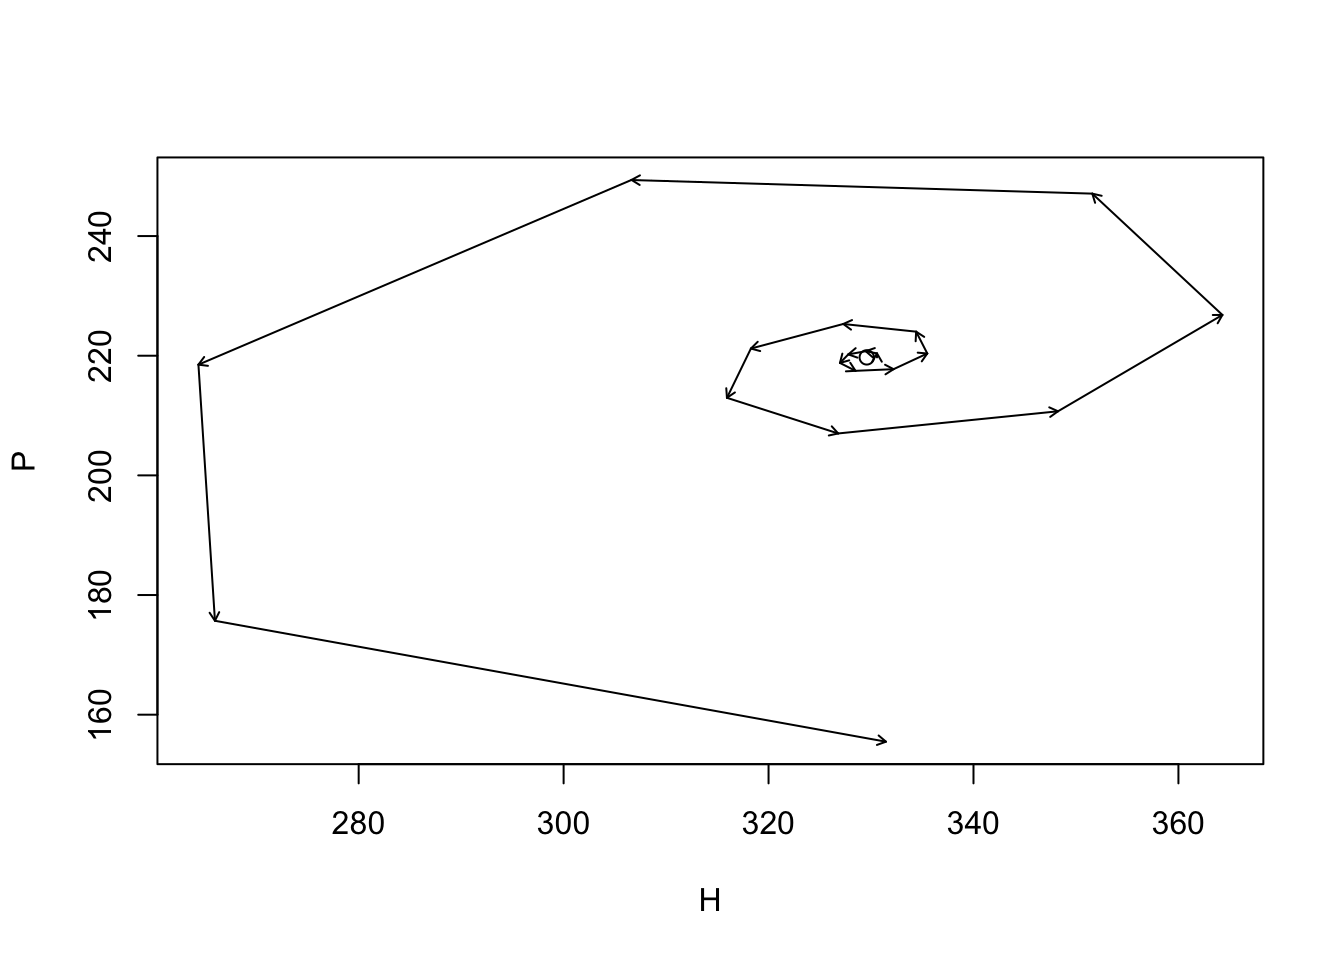
\includegraphics[scale=0.3]{Img/unnamed-chunk-114-1.png}
            \caption{Dinâmica do equilíbrio}
        \end{figure}
        
\newpage

\section{Referências}

(1) LIMA, Ernesto; FERREIRA, Cláudia; GODOY, Wesley. Ecological Modeling and Pest Population Management: a Possible and 
Necessary Connection in a Changing World. Neotropical Entomology, Botucatu, v. 38, n. 6, p. 699 - 707, nov/dec. 2009.

\medskip

(2) Alharbi, W., Sandhu, S.K., Areshi, M. et al. Ecological Modeling and Pest Population Management. Sci Rep 12, 15023 (2022). https://doi.org 10.1038/s41598-022-18120-z

\medskip

(3) HOVESTADT Thomas. Multiple host use and the dynamics of host switching in host–parasite systems. Insect Conservation and Diversity, Wallingford, v. 12, p. 511 - 522, 2019.

\medskip

(4) Mills, N.J., Getz, W.M. Modelling the biological control of insect pests: a review of host-parasitoid models. Mathematical Biology Group. 2018. Disponível em: https://www.colorado.edu/project/mathbio/2018/
05/02/host-parasitoid-models. Acesso em: 12 de set. de 2022. 

\medskip

(5) STEVENS Hank. Primer of Ecology using R. 2022. Disponível em: https://hankstevens.github.io/Pri
mer-of-Ecology/host-parasitoid-relations.html. Acesso em: 12 de set. de 2022.


\include{Introdução}
\include{Trabalhos}
\include{Metodologia}
\include{Referências}



\end{document}